\documentclass[11pt]{article}
\usepackage[utf8]{inputenc}
\usepackage[margin=1in]{geometry}
\usepackage{amsmath}
\usepackage[hidelinks]{hyperref}
\usepackage{enumitem}
\usepackage{tikz}
\usetikzlibrary{matrix,backgrounds}
\usetikzlibrary{patterns, calc}
\usepackage{pgfplots}
\pgfplotsset{compat=1.18}
\usepgfplotslibrary{fillbetween}
\tikzset{
  cell/.style={draw, minimum width=8mm, minimum height=8mm, anchor=center, font=\small},
  matrix border/.style={draw, line width=0.8pt}
}

\begin{document}

\begin{title}{\textbf{Computer Vision Series Summary}\\ \large Based on the Computerphile Lectures by Dr. Mike Pound}
\end{title}
\date{}

\maketitle
\newpage
\tableofcontents
\newpage
\section{Introduction}
This document provides a technical overview of the Computer Vision series produced by Computerphile. The series traces the evolution of the field from basic pixel manipulation (digital signal processing) to high-level object recognition using Deep Learning.

\newpage

\section{Fundamentals: Filters, Pixels, and Edges}

The foundation of computer vision is the \textbf{Convolution} (\texttt{Kernel Convolution}) which is obvious since the basic model of data is a signal and, thus, can be convoluted with the LTI filter to process the image. 

A computer treats an image as a matrix of intensity values. To process it, it uses a \textbf{Kernel} (a small odd sized matrix, e.g., a centered $3 \times 3$, representing the impulse response of the filter). The kernel slides (i.e. the shifting that exists in convolution) across the image. At each position, a "weighted sum" of the pixel and its neighbors (depending on the size of the kernel) is calculated. For example, a kernel filled with 1s (and \textbf{normalized} so the image doesn't get brighter or darker) acts as a \textbf{Mean Blur}. This is essential for removing high-frequency noise before performing edge detection. 

In figure~\ref{fig:edge-handling}, you will notice a very common situation. At the edges, some cells of the kernel will have no pixels to overlap with, at this point you need to take a decision either by ignore those ones and normalize the only effective ones, wrap the image around, or duplicate the edge ones. Nevertheless, that edge is a pixel in 5 to 10 megapixel image; it won't make that much of a difference.

\begin{figure}[htbp]
\centering
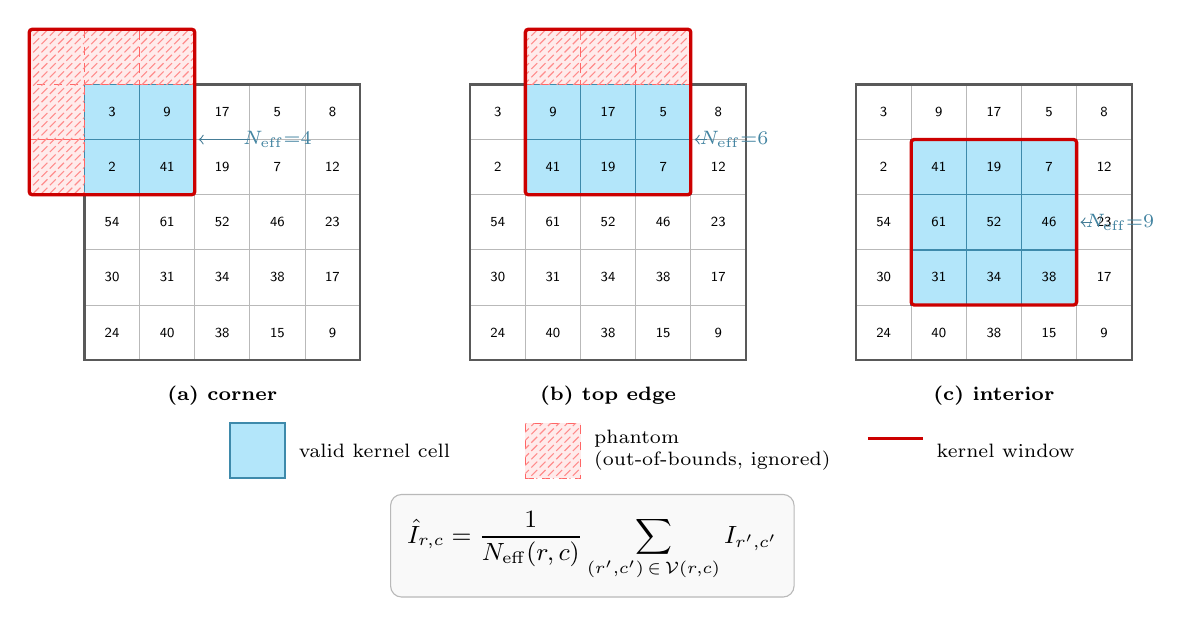
\begin{tikzpicture}[
  % base cell style
  cs/.style     = {minimum width=0.7cm, minimum height=0.7cm,
                   outer sep=0, inner sep=0, draw=gray!55,
                   font=\tiny\sffamily, line width=0.3pt},
  % plain image cell
  img/.style    = {cs, fill=white},
  % valid kernel cell (falls inside the image)
  valid/.style  = {cs, fill=cyan!30, draw=cyan!65!black, line width=0.55pt},
  % phantom kernel cell (falls outside the image – ignored)
  phantom/.style= {cs, draw=red!60, dashed, fill=red!8,
                   postaction={pattern=north east lines, pattern color=red!45}},
]

% ──────────────────────────
%  Helper macro: draws one 5×5 image grid.
%  Used with a surrounding \begin{scope}[xshift=...].
% ──────────
\newcommand{\imagegrid}{%
  \foreach \r/\c/\v in {
    0/0/3,  0/1/9,  0/2/17, 0/3/5,  0/4/8,
    1/0/2,  1/1/41, 1/2/19, 1/3/7,  1/4/12,
    2/0/54, 2/1/61, 2/2/52, 2/3/46, 2/4/23,
    3/0/30, 3/1/31, 3/2/34, 3/3/38, 3/4/17,
    4/0/24, 4/1/40, 4/2/38, 4/3/15, 4/4/9}
    \node[img] at ({0.7*\c},{-0.7*\r}) {\v};
  % image boundary
  \draw[black!65, thick] (-0.35,0.35) rectangle (3.15,-3.15);
}


% ═══════════════════════════════
%  PANEL (a) – 3×3 kernel at the top-left CORNER
%              Kernel spans rows {-1,0,1} × cols {-1,0,1}
%              Valid: 4 cells    Phantom: 5 cells
% ═══════════════════
\begin{scope}

  \imagegrid

  % valid cells (rows 0–1, cols 0–1)
  \foreach \r/\c/\v in {0/0/3, 0/1/9, 1/0/2, 1/1/41}
    \node[valid] at ({0.7*\c},{-0.7*\r}) {\v};

  % phantom cells (outside image boundary)
  \foreach \r/\c in {-1/-1, -1/0, -1/1, 0/-1, 1/-1}
    \node[phantom] at ({0.7*\c},{-0.7*\r}) {};

  % 3×3 kernel window border
  \draw[red!80!black, very thick, rounded corners=1pt]
    (-1.05,-1.05) rectangle (1.05,1.05);

  % annotation: effective count
  \node[cyan!60!black, font=\scriptsize\bfseries] at (2.1,-0.35)
    {$N_{\mathrm{eff}}{=}4$};
  \draw[cyan!55!black, ->, thin] (1.75,-0.35) -- (1.1,-0.35);

  \node[font=\scriptsize\bfseries, anchor=north] at (1.4,-3.35)
    {(a) corner};

\end{scope}
% ═══════════════════
%  PANEL (b) – 3×3 kernel at the TOP EDGE (centered on col 2)
%              Kernel spans rows {-1,0,1} × cols {1,2,3}
%              Valid: 6 cells    Phantom: 3 cells
% ═══════════
\begin{scope}[xshift=4.9cm]

  \imagegrid

  % valid cells (rows 0–1, cols 1–3)
  \foreach \r/\c/\v in {0/1/9, 0/2/17, 0/3/5, 1/1/41, 1/2/19, 1/3/7}
    \node[valid] at ({0.7*\c},{-0.7*\r}) {\v};

  % phantom cells (row -1, cols 1–3)
  \foreach \c in {1,2,3}
    \node[phantom] at ({0.7*\c},0.7) {};

  % kernel window border
  \draw[red!80!black, very thick, rounded corners=1pt]
    (0.35,1.05) rectangle (2.45,-1.05);

  \node[cyan!60!black, font=\scriptsize\bfseries] at (3.0,-0.35)
    {$N_{\mathrm{eff}}{=}6$};
  \draw[cyan!55!black, ->, thin] (2.65,-0.35) -- (2.5,-0.35);

  \node[font=\scriptsize\bfseries, anchor=north] at (1.4,-3.35)
    {(b) top edge};

\end{scope}

% ═════════════════════════
%  PANEL (c) – 3×3 kernel fully in the INTERIOR (centered on row 2, col 2)
%              Kernel spans rows {1,2,3} × cols {1,2,3}
%              Valid: 9 cells    Phantom: 0 cells
% ═══════════════════════════
\begin{scope}[xshift=9.8cm]

  \imagegrid

  % all 9 kernel cells are valid
  \foreach \r/\c/\v in {1/1/41,1/2/19,1/3/7,
                         2/1/61,2/2/52,2/3/46,
                         3/1/31,3/2/34,3/3/38}
    \node[valid] at ({0.7*\c},{-0.7*\r}) {\v};

  % kernel window border
  \draw[red!80!black, very thick, rounded corners=1pt]
    (0.35,-0.35) rectangle (2.45,-2.45);

  \node[cyan!60!black, font=\scriptsize\bfseries] at (3.0,-1.4)
    {$N_{\mathrm{eff}}{=}9$};
  \draw[cyan!55!black, ->, thin] (2.65,-1.4) -- (2.5,-1.4);

  \node[font=\scriptsize\bfseries, anchor=north] at (1.4,-3.35)
    {(c) interior};

\end{scope}

% ───────────────────────────
%  Legend
% ────────────────
\node[cs, fill=cyan!30, draw=cyan!65!black, line width=0.55pt] at (1.85,-4.3) {};
\node[font=\scriptsize, anchor=west] at (2.25,-4.3) {valid kernel cell};

\node[cs, draw=red!60, dashed, fill=red!8,
      postaction={pattern=north east lines, pattern color=red!45}] at (5.6,-4.3) {};
\node[font=\scriptsize, anchor=west, align=left] at (6.0,-4.3)
  {phantom \\ (out-of-bounds, ignored)};

\draw[red!80!black, very thick] (9.6,-4.15) -- (10.3,-4.15);
\node[font=\scriptsize, anchor=west] at (10.35,-4.3) {kernel window};

% ─────────────────────
%  General averaging formula
% ─────────────────
\node[draw=gray!55, rounded corners=4pt, fill=gray!5,
      inner sep=6pt, font=\small, anchor=north]
  at (6.1,-4.85)
  {$\displaystyle
     \hat{I}_{r,c}
       = \frac{1}{N_{\mathrm{eff}}(r,c)}
         \sum_{(r',c')\,\in\,\mathcal{V}(r,c)} I_{r',c'}
   $};

\end{tikzpicture}
\caption{Edge handling for averaging filters via adaptive normalization.
Rather than zero-padding, the output pixel $\hat{I}_{r,c}$ is divided only by
$N_{\mathrm{eff}}(r,c)$, the number of kernel positions that lie within the
valid image region~$\mathcal{V}(r,c)$.}
\label{fig:edge-handling}
\end{figure}

%%%%%%%%%%%%%%%%%%%%%%%%%%%%%%%%%%%%%%%%%%

\noindent\textbf{Disclaimer:} the output of the kernel should be outputted to a different image or, in computer words, a different matrix, because if the image original matrix is overwritten as we go, it will mess up the math as this pixel is a neighbor to other upcoming pixels.

\section{Gaussian Blur}
Gaussian blur (normal distribution) is extremely common, perhaps the most common blur; it is a bit more controlled and edge preserving that a mean blur.

\noindent A normal distribution is essentially a bell curve shaped by its mean and standard deviation where the standard deviation, $\sigma$, is the average squared distance from the mean of all the points.

\begin{center} % Use the center environment for page centering
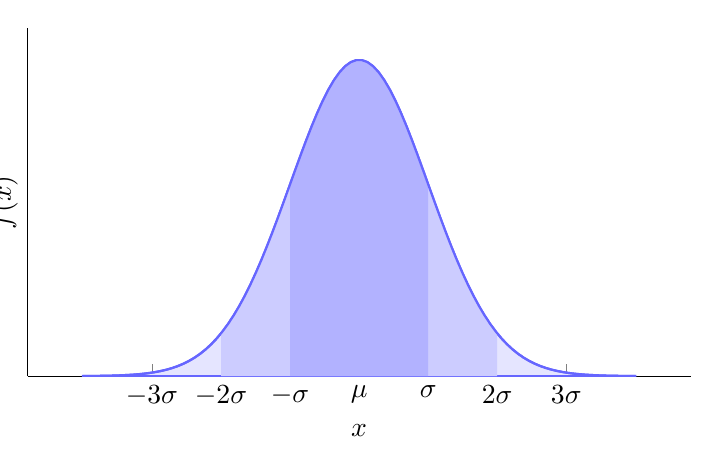
\begin{tikzpicture}[trim axis left, trim axis right]
\begin{axis}[
    no markers, 
    domain=-4:4, 
    samples=100,
    ymin=0,
    axis lines*=left, 
    xlabel=$x$, 
    ylabel={$f(x)$},
    height=6cm, 
    width=10cm,
    xtick={-3,-2,-1,0,1,2,3},
    xticklabels={$-3\sigma$,$-2\sigma$,$-\sigma$,$\mu$,$\sigma$,$2\sigma$,$3\sigma$},
    ytick=\empty,
    % These two lines ensure the labels don't "push" the plot
    ylabel style={overlay}, 
    yticklabel style={overlay}
    ]
    % Fill 3-sigma
    \addplot [name path=curve, thick, fill=blue!10, draw=blue!60] {1/(sqrt(2*pi))*exp(-x^2/2)} \closedcycle;
    
    % Fill 2-sigma
    \addplot [name path=curve2, fill=blue!20, draw=none, domain=-2:2] {1/(sqrt(2*pi))*exp(-x^2/2)} \closedcycle;
    
    % Fill 1-sigma
    \addplot [name path=curve3, fill=blue!30, draw=none, domain=-1:1] {1/(sqrt(2*pi))*exp(-x^2/2)} \closedcycle;

    % Redraw the curve on top
    \addplot [thick, draw=blue!60] {1/(sqrt(2*pi))*exp(-x^2/2)};
\end{axis}
\end{tikzpicture}
\end{center}

\subsection{Video 2: Finding the Edges (Sobel Operator)}
Edges occur where there is a sharp change in pixel intensity.
\begin{itemize}
    \item \textbf{Sobel Kernels:} Two kernels ($G_x$ and $G_y$) are used to find horizontal and vertical gradients.
    \item \textbf{The Math:} The total gradient magnitude $G$ is calculated as:
    \begin{equation}
        G = \sqrt{G_x^2 + G_y^2}
    \end{equation}
    \item \textbf{Output:} An image where edges are bright and flat areas are black.
\end{itemize}

\subsection{Video 3: Canny Edge Detector}
The Canny detector is a multi-stage process designed for "optimal" edge detection:
\begin{enumerate}[noitemsep]
    \item \textbf{Gaussian Blur:} To suppress noise.
    \item \textbf{Sobel Gradient:} To find edge candidates.
    \item \textbf{Non-Maximum Suppression:} "Thins" edges by looking for the peak of the gradient.
    \item \textbf{Hysteresis Thresholding:} Uses two thresholds to keep weak edges only if they are connected to strong ones.
\end{enumerate}

\section{Feature Extraction and Shape Detection}

\subsection{Video 4: Hough Transform}
The Hough Transform solves the problem of grouping edge pixels into mathematical shapes.
\begin{itemize}
    \item \textbf{Parameter Space:} Points in the $(x, y)$ image space are mapped to curves in $(\rho, \theta)$ space.
    \item \textbf{Voting:} Each edge pixel "votes" for all possible lines it could belong to.
    \item \textbf{Consensus:} Intersection points in Hough space represent the most likely lines or circles in the original image.
\end{itemize}

\subsection{Video 5: Template Matching}
A fundamental approach to finding objects.
\begin{itemize}
    \item \textbf{Method:} Sliding a small "template" image over a larger search image.
    \item \textbf{Metrics:} Calculated using \textbf{Sum of Squared Differences (SSD)} or \textbf{Cross-Correlation}.
    \item \textbf{Limitation:} It is highly sensitive to changes in scale, lighting, and rotation.
\end{itemize}

\subsection{Video 6: Interest Points (Harris Corner Detection)}
Corners are more robust features than edges.
\begin{itemize}
    \item \textbf{Mechanism:} A corner is defined as a region where the intensity changes significantly in all directions when the observation window is shifted.
    \item \textbf{The Math:} Uses the eigenvalues ($\lambda_1, \lambda_2$) of the local gradient matrix. If both are large, the point is a corner.
\end{itemize}

\section{Advanced Recognition and AI}

\subsection{Video 7: SIFT (Scale Invariant Feature Transform)}
SIFT is the pinnacle of "classic" feature extraction.
\begin{itemize}
    \item \textbf{Invariance:} It identifies "Keypoints" that remain recognizable even if the object is rotated, resized, or seen from a different angle.
    \item \textbf{Descriptor:} Each keypoint is assigned a unique vector (descriptor) based on local gradients, allowing for robust matching between different images.
\end{itemize}

\subsection{Video 8: Searching for Objects (Viola-Jones)}
The classic real-time face detection algorithm.
\begin{itemize}
    \item \textbf{Haar Features:} Looks for simple contrast patterns (e.g., eyes are darker than the nose bridge).
    \item \textbf{The Cascade:} A sequence of increasingly complex "weak classifiers." If an image sub-region fails the first simple test, it is discarded immediately, saving massive computation.
\end{itemize}

\subsection{Video 9: Deep Learning / Convolutional Neural Networks (CNNs)}
The shift from "Hand-Crafted Features" to "Learned Features."
\begin{itemize}
    \item \textbf{Architecture:} Multi-layered networks that learn the kernels (filters) themselves through backpropagation.
    \item \textbf{Hierarchy:} Early layers learn simple edges; middle layers learn parts (ears, noses); final layers recognize the object (Cat vs. Dog).
\end{itemize}

\end{document}
